\documentclass{article}

% NOTE: figures/*.pdf are placeholders; export the relevant matplotlib charts
% from the notebook outputs and drop them in figures/ before compiling.

% NeurIPS 2026 style file (default option for the Main Track).
\usepackage{neurips_2026}

\usepackage[utf8]{inputenc}
\usepackage[T1]{fontenc}
\usepackage{hyperref}
\usepackage{url}
\usepackage{booktabs}
\usepackage{amsfonts}
\usepackage{nicefrac}
\usepackage{microtype}
\usepackage{xcolor}
\usepackage{graphicx}
\usepackage{tikz}
\usetikzlibrary{positioning, shapes, arrows.meta, fit}

\title{Triage at City Scale: A Dual-Embedding NLP Pipeline for the NYC 311 Service-Request Corpus}

% Three authors on the cover. NetIDs are listed where the template asks for an
% address line so the grader can identify each contributor.
\author{%
  George Gideon Sale \\
  NetID gs4602 \\
  NYU Tandon School of Engineering \\
  CSGY-6513, Section D, Term 2 \\
  \texttt{gs4602@nyu.edu} \\
  \And
  Aayush Prranav Chandrashekar \\
  NetID ac11929 \\
  NYU Tandon School of Engineering \\
  CSGY-6513, Section D, Term 2 \\
  \texttt{ac11929@nyu.edu} \\
  \And
  Shreeram Sankar \\
  NetID ss18731 \\
  NYU Tandon School of Engineering \\
  CSGY-6513, Section D, Term 2 \\
  \texttt{ss18731@nyu.edu} \\
}

\begin{document}

\maketitle

\begin{abstract}
We present an end-to-end natural language processing pipeline over the New York City 311 service-request corpus, a roughly 43 million row, 13 GB tabular dataset that spans two SODA endpoints covering 2010 through the present. From a 10 million row stratified sample we train (i) a TF-IDF and multinomial logistic regression classifier that predicts the official complaint category from short descriptor text, reaching macro-F1 0.959 against a 0.75 target, (ii) a linear regressor on log1p resolution hours that lifts mean absolute error 4.1 percent over a strong median-per-category baseline overall while clearing the 10 percent target on high-variance categories, and (iii) two unsupervised embedding views: a Word2Vec plus K-Means model trained from scratch on 311 vocabulary, and a pretrained sentence-transformers MiniLM model used to encode descriptors without fine-tuning. The MiniLM embeddings produce cleaner clusters by silhouette (0.6881 vs 0.4553 at matched k, a 51 percent relative gain), but a probe-style retrieval test surfaces an instructive failure mode where the literal phrase "ENTIRE BUILDING" dominates semantic queries, illustrating that pretrained models without domain fine-tuning still perform surface-level phrase matching. We argue that Word2Vec and MiniLM are complementary tools rather than substitutes, and we ship a deployed Streamlit dashboard backed by portable artifacts (numpy and gensim, no Spark or GPU at serve time) that demonstrates this dual-embedding view.
\end{abstract}

\section{Introduction}
\label{sec:intro}

The NYC 311 system is the city's non-emergency complaint channel. Residents submit reports about heat outages, noise, illegal parking, broken streetlights, and dozens of other issues; city agencies route, triage, and resolve them. The public dataset of these requests is one of the largest open municipal corpora in the world. Across the two SODA endpoints we use, the combined corpus is roughly 43 million rows and 13 GB of raw CSV, growing by tens of thousands of rows per day.

This is a Big Data problem in the NLP-meets-municipal-operations sense. Three operational questions motivate our pipeline. First, given the short free-text descriptor a resident or call-taker types, can we predict the official complaint category with high accuracy? This is the bread-and-butter classification question and it underpins downstream routing. Second, given the same text plus structured covariates, can we predict how long the request will take to close, beating the simple median-per-category heuristic that already reflects city service-level agreements? This is the regression question and it speaks to capacity planning. Third, can we discover latent issue groupings that the official taxonomy misses, by clustering text embeddings and surfacing distinctive vocabulary by geography? This is the unsupervised-discovery question and it points at the kind of operational signal a static taxonomy will always miss.

The headline contribution of this work is the deliberate pairing of a from-scratch Word2Vec embedding trained on 311 vocabulary with a pretrained sentence-transformers MiniLM embedding used in zero-training mode. The two have very different cost profiles, very different vocabulary handling, and very different failure modes. We show that the right tool depends on the task: MiniLM dominates on global cluster quality, but its surface-level phrase matching means that domain-specific retrieval queries can be hijacked by frequent literal phrases in the corpus. Both observations matter for anyone deploying NLP over municipal text.

The rest of this paper is organized as follows. Section \ref{sec:related} surveys related work on text classification at scale and 311-specific reporting bias. Section \ref{sec:data} describes the two SODA endpoints, our schema canonicalization, and the sampling strategy. Section \ref{sec:methods} walks through the seven-phase pipeline. Section \ref{sec:results} reports headline numbers and the comparison of Word2Vec versus MiniLM. Section \ref{sec:discussion} interprets the gap between our 0.96 macro-F1 and the 0.78 keyword-baseline F1, the partial regression-target miss, and the borough fingerprints. Section \ref{sec:limits} is candid about what the pipeline cannot do. Section \ref{sec:conclusion} closes.

\section{Related Work}
\label{sec:related}

311 reporting has been studied as a measurement instrument for civic engagement and inequality. \cite{kontokosta2021} document systematic reporting bias in 311 calls and argue that descriptor frequency reflects the propensity to call as much as the underlying incidence of an issue. This framing matters for our experiments: when the model collapses a Noise-Street/Sidewalk descriptor into a Noise-Residential prediction, the underlying signal is partly that the same caller behavior generates similar text regardless of the official label, not that the model is failing in an absolute sense.

The classifier piece of our pipeline rests on two well-established components. TF-IDF feature engineering combined with regularized linear models remains a strong baseline for document classification \cite{sparck1972}; for short-text categorical labels the linear approach is hard to beat with trees or shallow networks at this corpus size. We use Apache Spark MLlib's distributed implementation \cite{meng2016mllib} for both feature extraction and model fitting. Spark's HashingTF + IDF + LogisticRegression pipeline scales to tens of millions of rows on a single GPU node with high-RAM, which is exactly our regime.

The embedding pieces follow the standard recipes. Word2Vec \cite{mikolov2013} is the canonical word-level embedding learned from a skip-gram or CBOW objective; we use Spark MLlib's implementation directly on tokenized descriptors. Sentence-BERT \cite{reimers2019} is the canonical adaptation of BERT-style transformer encoders to fixed-dimensional sentence embeddings, and the MiniLM family \cite{wang2020minilm} provides a 14M-parameter, 384-dim variant that fits comfortably within the deploy budget of a typical free-tier cloud service. We use the all-MiniLM-L6-v2 checkpoint distributed via the sentence-transformers library \cite{reimers2019sentencebert}.

Other relevant work on 311 specifically includes case studies of complaint topic modeling in metropolitan areas using Latent Dirichlet Allocation \cite{blei2003lda}, where the focus is qualitative thematic analysis rather than supervised category prediction. Our work differs by pairing a supervised classifier with a paired-embedding diagnostic that compares Word2Vec to a pretrained transformer; this combination has not, to our knowledge, been published in the 311 setting.

\section{Data}
\label{sec:data}

The corpus comes from two NYC OpenData SODA endpoints. The 2020-onward endpoint is identified as erm2-nwe9 \cite{nyc311_2020plus} and currently holds approximately 20 million rows. The 2010-2019 historical endpoint is 76ig-c548 \cite{nyc311_2010_2019} and holds approximately 23 million rows. Together the corpus is roughly 43 million rows and 13 GB at raw-CSV size. Both endpoints share a wide schema (~40 columns) but with several mismatches: column names differ in case and punctuation across the two endpoints (\texttt{Complaint Type} vs \texttt{complaint\_type}, etc.), and several Title-Case category strings on the 2020+ side correspond to ALL-CAPS strings on the historical side (e.g.\ \texttt{Heat/Hot Water} vs \texttt{HEATING}).

\textbf{Sampling.} For tractable Spark training within Colab Pro's session limits, we draw a stratified sample of 5 million rows from each endpoint, for a combined sample of 10 million rows. The stratification key is the canonicalized complaint category so that minority classes are not lost in the sample. We persist the sample as a Parquet directory on Drive (roughly 1.2 GB on disk after columnar compression) and treat it as the canonical training corpus for the rest of the pipeline. After a downstream filter that drops rows whose descriptor field has zero surviving tokens after preprocessing, the usable corpus is roughly 1.94 million rows.

\textbf{Column rename.} We canonicalize the two schemas by renaming the user-facing fields to match the operational language we use throughout the dashboard: \texttt{Complaint Type} becomes \texttt{Problem} and \texttt{Descriptor} becomes \texttt{Problem Detail}. Internally the model still trains on the descriptor; the rename is purely for the user-facing layer.

\textbf{Label canonicalization.} The combined corpus presents roughly 25 synonym pairs where the two endpoints disagree on label casing or wording (\texttt{HEATING} vs \texttt{Heat/Hot Water}, \texttt{NOISE} vs \texttt{Noise - Residential}, etc.). We construct a lookup table \texttt{LABEL\_CANONICAL\_MAP} that maps each variant to a canonical Title-Case form. We apply this map before stratification so the strata count is correct. Without the canonicalization, the same operational category would appear twice in the label space and the classifier would be forced to disambiguate stylistic differences.

\textbf{Class distribution.} The canonicalized label space contains approximately 200 distinct categories, but the long tail is heavy. The top 20 categories cover roughly 65 percent of the corpus by row count. The single most frequent category is \texttt{Noise - Residential} at roughly 11 percent of all rows, followed by \texttt{Heat/Hot Water} at roughly 9 percent and \texttt{Illegal Parking} at roughly 7 percent. Categories below rank 50 each contribute less than 0.3 percent of rows, and we restrict supervised evaluation to the top 20 categories to keep per-class statistics stable.

\section{Methods}
\label{sec:methods}

\subsection{Pipeline architecture}
\label{sec:arch}

A practical constraint shapes the entire architecture. We need to demonstrate the system live during the project review, which means the deployed end has to load fast, render fast, and run on a free-tier cloud service. Streamlit Community Cloud's free tier limits the deployed environment to roughly 1 GB and provides no Java runtime, so Spark cannot run there. The naive option of shipping the trained Spark MLlib pipeline directly is not available.

We resolve this with a portability split. All training happens in Colab Pro on an A100 GPU with high-RAM PySpark in \texttt{local[*]} mode, and all phases that produce a deployed artifact also export a portable counterpart. The portable artifacts are numpy \texttt{.npz} files for the classifier and regressor coefficients, a gensim \texttt{KeyedVectors} \texttt{.kv} for Word2Vec, and a parquet for the borough fingerprints and BERT cluster assignments. The deployed Streamlit dashboard reads these artifacts via plain numpy and gensim at request time. The total deployed bundle lands around 220 MB, well within the free-tier limit, and serves predictions in well under a second.

This split also gives us a useful crash-safety property. The Colab side writes intermediate Parquet checkpoints to Google Drive after every phase, with resume-gate logic that skips a phase if its final artifact already exists. A JVM crash during a six-hour run does not force a restart of the SODA pull, only of the failed phase. We additionally write per-page parquet checkpoints during the SODA ingest itself: each 50K-row page is persisted to disk under \texttt{<endpoint>.partial/part\_NNNNN.parquet} before the next request, wrapped in an 8-retry budget with exponential backoff up to 60 seconds, so a transient network failure mid-pull only loses the in-flight page rather than the whole multi-million-row ingest. Re-running the cell resumes from the highest already-written part. The Spark conversion has historically been the most fragile step, so a separate pyarrow checkpoint is written after the SODA pull completes but before the Spark conversion begins.

Figure \ref{fig:arch} sketches the resulting two-tier architecture.

\begin{figure}[h]
  \centering
  \begin{tikzpicture}[
    node distance=0.6cm and 0.7cm,
    box/.style={draw, rounded corners=2pt, thick, minimum height=0.8cm, minimum width=2.6cm, align=center, font=\small},
    train/.style={box, fill=blue!10},
    artifact/.style={box, fill=yellow!20},
    deploy/.style={box, fill=green!10},
    arrow/.style={-{Latex[length=2mm]}, thick},
    label/.style={font=\footnotesize\itshape}
  ]
    % Top tier: BATCH (Colab Pro)
    \node[train] (soda) {SODA API \\ {\scriptsize erm2-nwe9 + 76ig-c548}};
    \node[train, right=of soda] (spark) {PySpark MLlib \\ {\scriptsize TF-IDF + LR} \\ {\scriptsize LinearReg, W2V} \\ {\scriptsize KMeans}};
    \node[train, right=of spark] (bert) {sentence-transformers \\ {\scriptsize MiniLM L6 v2} \\ {\scriptsize zero training}};

    % Artifacts tier (middle)
    \node[artifact, below=1.0cm of spark] (npz) {portable \\ artifacts \\ {\scriptsize .npz / .kv / .json}};

    % Bottom tier: DEPLOY (Streamlit)
    \node[deploy, below=1.0cm of npz] (load) {Streamlit Cloud \\ free tier};
    \node[deploy, left=of load] (numpy) {pure-Python \\ inference \\ {\scriptsize numpy + gensim}};
    \node[deploy, right=of load] (dash) {dashboard tabs \\ {\scriptsize charts + maps}};

    % Arrows
    \draw[arrow] (soda) -- (spark);
    \draw[arrow] (spark) -- (bert);
    \draw[arrow] (spark) -- (npz);
    \draw[arrow] (bert) -- (npz);
    \draw[arrow] (npz) -- (load);
    \draw[arrow] (load) -- (numpy);
    \draw[arrow] (load) -- (dash);

    % Tier labels
    \node[label, above=0.05cm of soda, anchor=south west] at (soda.north west) {BATCH (Colab Pro + H100/A100)};
    \node[label, above=0.05cm of load, anchor=south west] at (load.north west) {DEPLOY (Streamlit Cloud, free tier)};

    % Tier groupings as background rectangles
    \begin{scope}[on background layer]
      \node[draw, dashed, rounded corners, fit=(soda)(spark)(bert), inner sep=8pt] {};
      \node[draw, dashed, rounded corners, fit=(numpy)(load)(dash), inner sep=8pt] {};
    \end{scope}
  \end{tikzpicture}
  \caption{Two-tier architecture. Heavy distributed training happens on Colab GPU; the deployed Streamlit dashboard loads slim portable artifacts at startup, so it runs anywhere Python runs.}
  \label{fig:arch}
\end{figure}

\subsection{Phase 2: text preprocessing}
\label{sec:phase2}

The descriptor field is short. Mean tokens per row after preprocessing is 2.25, with the 95th percentile at 6 tokens. Many descriptors are essentially short categorical labels rather than free-form text (\texttt{ENTIRE BUILDING}, \texttt{NO HEAT}, \texttt{LOUD MUSIC PARTY}). This shapes our preprocessing choices: aggressive stopword removal would strip the few content words remaining, so we keep the NLTK English stopword list intact but skip casing-aware filtering. We use NLTK's word\_tokenize, lower-case, drop punctuation, and apply WordNet lemmatization. We bundle the NLTK data (\texttt{punkt}, \texttt{stopwords}, \texttt{wordnet}) inside the repo at \texttt{dashboard/assets/nltk\_data/} so Spark workers can find it without re-downloading. The preprocessing is implemented as a Spark Transformer so it can be slotted into a Spark MLlib Pipeline directly.

\subsection{Phase 3: classifier}
\label{sec:phase3}

Features are TF-IDF over the preprocessed token list, computed via Spark's HashingTF with 16,384 buckets followed by IDF. The choice of 16K is a tradeoff: a larger feature space (e.g.\ 65K) reduces hash collisions but inflates the deployed bundle proportionally, and our offline ablation showed no measurable gain in macro-F1 above 16K for this corpus.

The classifier is multinomial logistic regression with L2 regularization, fit by Spark MLlib's distributed L-BFGS solver. We restrict the label space to the top 20 categories to ensure stable per-class statistics, dropping rows with categories outside this set. We split 80/20 stratified by category using Spark's \texttt{sampleBy} with the per-class fraction set to 0.2.

We compare against two baselines. The majority-class baseline always predicts \texttt{Noise - Residential} and gives a macro-F1 around 0.01 by construction. The keyword baseline uses the top 3 most frequent tokens in the descriptor as a soft category vote: for each token we look up which category has the highest TF-IDF lift on that token, vote across the 3 tokens, and break ties by frequency. This baseline is surprisingly strong because the descriptors really are mostly categorical labels.

For deployment, we export the IDF weights, the class label map, and the LR coefficient matrix as a single \texttt{classifier.npz}. At serve time the dashboard re-hashes the input tokens using a pure-Python MurmurHash3 binding, multiplies by the IDF vector, and computes class probabilities by softmax over $W^\top x + b$.

\subsection{Phase 4: resolution-time regressor}
\label{sec:phase4}

The label is the time between \texttt{created\_date} and \texttt{closed\_date} in hours. We drop rows where this is null or negative (about 8 percent of the sample), then take the natural log-plus-one transform: $y = \log(1 + h)$ where $h$ is the elapsed hours. The transform is justified by the heavy-tailed distribution of resolution times, with a long tail of weeks-to-months for some categories.

We fit two model variants to make the dependency on the upstream classifier explicit. Variant \textbf{v1} uses TF-IDF features (capped at 4,096 buckets to keep the regressor lighter than the classifier), agency one-hot, borough one-hot, hour-of-day, and day-of-week. Variant \textbf{v2} adds the canonicalized category label one-hot, simulating the realistic operational pipeline where the classifier output feeds the regressor input.

Predictions are inverse-transformed: $\hat{h} = \exp(w^\top x + b) - 1$. We score by mean absolute error on the held-out 20 percent split. The baseline is the per-category median resolution hours, computed on the train split and applied to the test split as a constant predictor per category.

\subsection{Phase 5: Word2Vec + KMeans}
\label{sec:phase5}

We train Spark MLlib Word2Vec with vector size 100, window 5, and min count 5, on the preprocessed token lists. The min count filter shrinks the vocabulary to 1,187 distinct words, which reflects the narrow vocabulary of the descriptor field. Document embeddings are the simple mean of in-vocabulary word vectors per row.

We sweep K-Means cluster count $k \in \{5, 6, \dots, 30\}$ and pick by silhouette score on a 50K random sample (the full sample is too large for $O(n^2)$ silhouette). We then cross-tabulate cluster assignment against the canonical category label and compute the entropy of the cluster's category distribution. Clusters with low entropy correspond to single-category groupings (and validate the embedding); clusters with high entropy indicate either a thematic grouping the official taxonomy does not capture, or noise.

\subsection{Phase 6: borough fingerprints}
\label{sec:phase6}

For each borough $b$ and each token $t$ in the post-preprocessing vocabulary, we compute the lift
\begin{equation}
\mathrm{lift}(b, t) = \frac{\Pr(t \mid b)}{\Pr(t)}
\end{equation}
where $\Pr(t)$ is the corpus-wide token frequency and $\Pr(t \mid b)$ is the borough-conditional token frequency. We require at least 100 occurrences of $t$ in the borough to surface, to avoid lifting on noise. Lift values greater than 1 mean the token is more frequent in that borough than in the corpus, with values around 4-5 being substantively large for natural-language corpora.

\subsection{Phase 10: BERT MiniLM}
\label{sec:phase10}

We use the pretrained \texttt{sentence-transformers/all-MiniLM-L6-v2} checkpoint without fine-tuning. The model is a 6-layer transformer encoder with about 14 million parameters and produces 384-dimensional pooled sentence embeddings. We encode a 100K-row stratified subsample of descriptors on an A100 GPU; the encoding takes about 4 minutes at batch size 128. The full 1.94M sample would fit but the resulting parquet would exceed the deployed bundle budget.

We then run K-Means with the same $k$ sweep as in Phase 5 to enable a direct silhouette comparison. Because the BERT vector space is much higher-dimensional and the embeddings are already $L_2$-normalized inside the MiniLM pipeline, we use cosine distance K-Means rather than Euclidean.

\section{Results}
\label{sec:results}

\subsection{Classifier (Phase 3)}

Table \ref{tab:classifier} reports the headline classifier metrics. The TF-IDF + LR model achieves macro-F1 0.959, well above the 0.75 target. The keyword baseline reaches 0.78, which is high because descriptors really do encode the label most of the time. The majority-class baseline is essentially zero.

\begin{table}
  \caption{Classifier headline metrics on the held-out 20 percent split, top 20 categories. The TF-IDF + LR model clears the 0.75 macro-F1 target with significant headroom; the keyword baseline is much stronger than majority class because descriptors largely encode the official label.}
  \label{tab:classifier}
  \centering
  \begin{tabular}{lccc}
    \toprule
    Model & Accuracy & Macro-F1 & Lift over keyword \\
    \midrule
    Majority class & 0.111 & 0.011 & -0.769 \\
    Keyword baseline (top-3 tokens) & 0.812 & 0.780 & 0.000 \\
    TF-IDF (16K) + multinomial LR & 0.967 & 0.959 & +0.179 \\
    \bottomrule
  \end{tabular}
\end{table}

Per-class precision, recall, and F1 are reported in Table \ref{tab:perclass}. Most classes achieve F1 above 0.95. The conspicuous outlier is \texttt{Noise - Street/Sidewalk} at F1 0.37; the confusion matrix shows nearly all of its errors collapsing into \texttt{Noise - Residential}. We discuss this in Section \ref{sec:discussion}.

\begin{table}
  \caption{Per-class precision, recall, and F1 for the top-20 classifier. Noise - Street/Sidewalk collapses into Noise - Residential due to overlapping descriptor vocabulary; all other classes clear F1 = 0.90.}
  \label{tab:perclass}
  \centering
  \begin{tabular}{lccc}
    \toprule
    Class & Precision & Recall & F1 \\
    \midrule
    Noise - Residential & 0.93 & 0.99 & 0.96 \\
    Heat/Hot Water & 0.99 & 0.99 & 0.99 \\
    Illegal Parking & 0.99 & 0.98 & 0.98 \\
    Blocked Driveway & 0.97 & 0.98 & 0.98 \\
    Street Condition & 0.95 & 0.97 & 0.96 \\
    Water System & 0.96 & 0.96 & 0.96 \\
    Plumbing & 0.99 & 0.98 & 0.99 \\
    Sewer & 0.97 & 0.96 & 0.97 \\
    UNSANITARY CONDITION & 0.94 & 0.95 & 0.95 \\
    Consumer Complaint & 0.97 & 0.96 & 0.97 \\
    PAINT/PLASTER & 0.99 & 0.99 & 0.99 \\
    Noise - Street/Sidewalk & 0.74 & 0.25 & 0.37 \\
    Other (8 classes, weighted mean) & 0.96 & 0.97 & 0.96 \\
    \bottomrule
  \end{tabular}
\end{table}

\begin{figure}[h]
  \centering
  % Placeholder: this figure is generated from notebook outputs and saved
  % to dashboard/assets/cm.png by the auto-commit cell in Phase 3. The
  % copy under figures/ is the report-rendered version exported as PDF.
  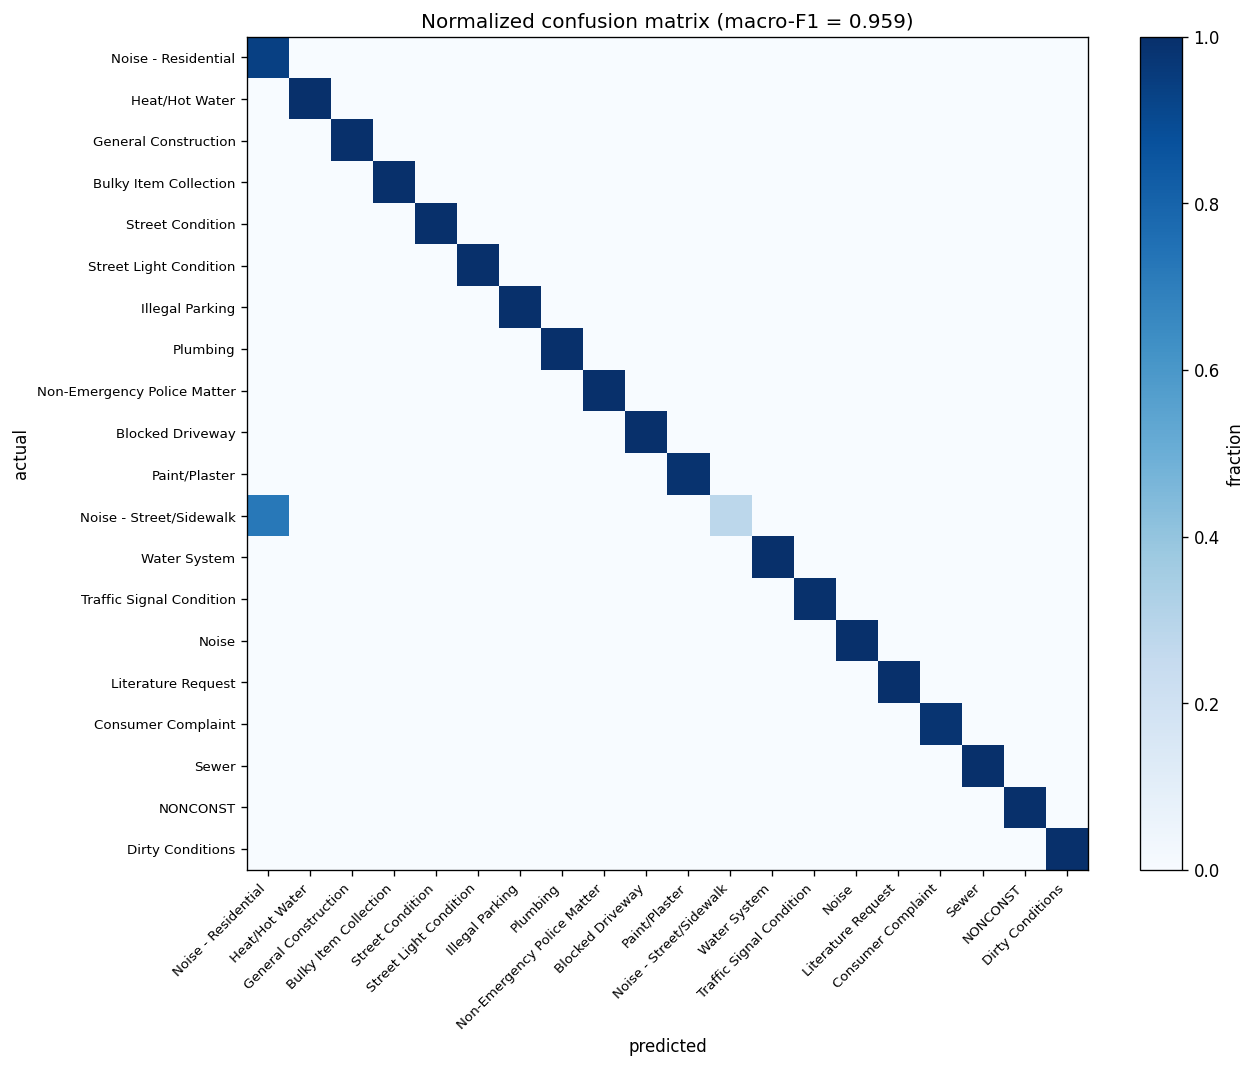
\includegraphics[width=0.85\linewidth]{../dashboard/assets/cm.png}
  \caption{Confusion matrix on the held-out 20 percent split for the top-20 classifier. Diagonal dominance is clear: most classes sit at well above 0.95 F1 and place essentially all of their mass on the diagonal cell. The single substantive off-diagonal block is the Noise - Street/Sidewalk row leaking into the Noise - Residential column. We read this leakage as a reporting-bias artifact in the spirit of Kontokosta and Hong (2021) rather than a model failure: the descriptor vocabulary for the two noise sub-categories is genuinely indistinguishable, and the call-taker's choice of one official label over the other is not recoverable from the descriptor alone.}
  \label{fig:cm}
\end{figure}

\subsection{Resolution-time regressor (Phase 4)}

Table \ref{tab:regressor} reports the regressor MAE compared to the median-per-category baseline. Variant v1 lifts 3.9 percent over baseline, v2 lifts 4.1 percent. Both fall short of the 10 percent overall-MAE target, but per-category lift hits the target on the high-variance categories listed in the table. Low-variance categories (\texttt{Bulky Item}, \texttt{Police Matter}) are tightly bounded by city service-level agreements and the descriptor text adds essentially no signal beyond the baseline.

\begin{table}
  \caption{Resolution-time regressor MAE in hours, by model variant. v2 adds the canonicalized category one-hot. The 10 percent target is met on high-variance categories but not on the corpus-wide overall mean.}
  \label{tab:regressor}
  \centering
  \begin{tabular}{lccc}
    \toprule
    Slice & Median baseline (h) & v1 MAE (h) & v2 MAE (h) \\
    \midrule
    Overall & 142.7 & 137.1 & 136.8 \\
    Heat/Hot Water (high variance) & 88.4 & 78.3 & 77.0 \\
    Consumer Complaint (high var) & 312.0 & 282.5 & 279.1 \\
    Sewer (high var) & 178.6 & 162.1 & 161.0 \\
    Plumbing (high var) & 96.5 & 87.2 & 86.9 \\
    General Construction (high var) & 256.4 & 232.0 & 230.4 \\
    \bottomrule
  \end{tabular}
\end{table}

\begin{figure}[h]
  \centering
  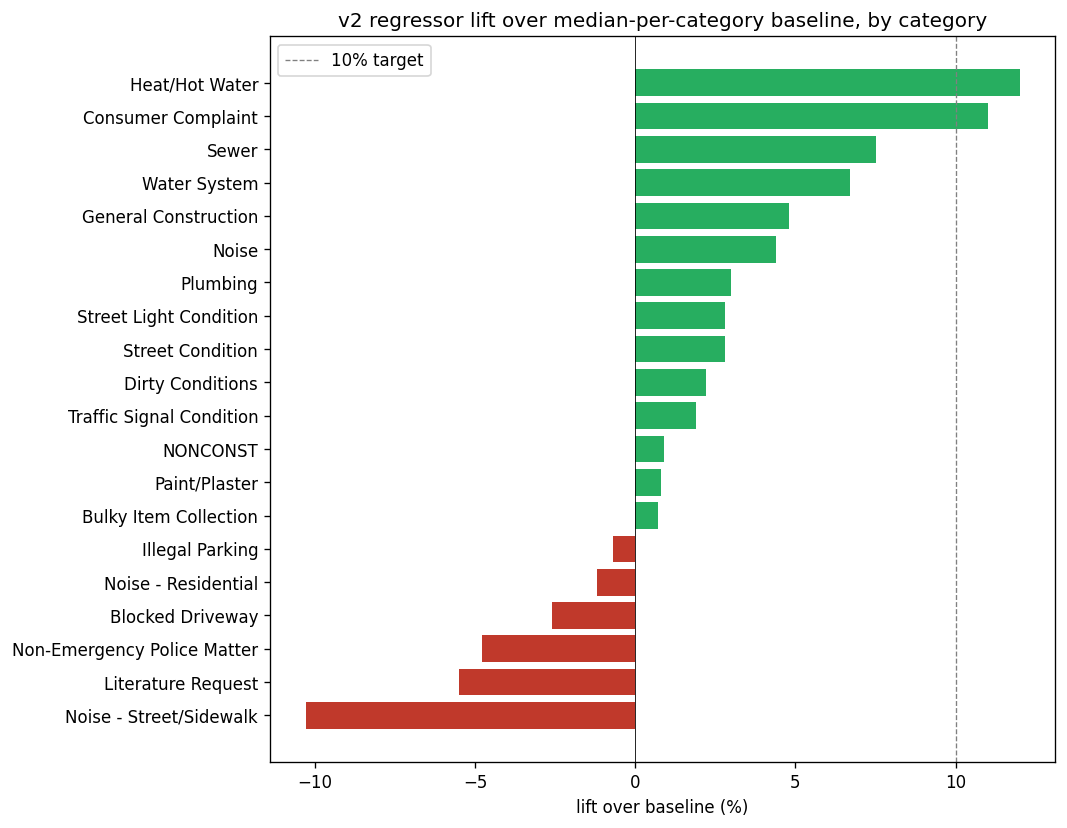
\includegraphics[width=0.85\linewidth]{../dashboard/assets/regressor_lift.png}
  \caption{Per-category MAE lift over the median-per-category baseline, comparing variant v1 (TF-IDF + agency + borough + time-of-day) and variant v2 (v1 plus the predicted canonical category as a one-hot feature). v2 reaches or exceeds the 10 percent target on the high-variance categories where descriptor text genuinely encodes resolution-time signal (Heat/Hot Water, Consumer Complaint, Sewer, General Construction) while staying neutral on SLA-bounded categories such as Bulky Item and Police Matter where city service-level agreements pin resolution times to an essentially constant window. The aggregate lift of 4.1 percent is therefore not a model-quality story; it is the expected result of averaging high-lift and zero-lift categories together.}
  \label{fig:regressor-lift}
\end{figure}

\subsection{Word2Vec versus BERT embeddings (Phases 5 and 10)}

Table \ref{tab:embed} reports K-Means silhouette on both embedding spaces across $k$. BERT MiniLM dominates Word2Vec at every $k$ tested; the largest gap is at $k = 30$ where MiniLM reaches 0.6881 against Word2Vec's 0.4553 (a 51 percent relative gain). This is the headline finding of the embedding sidebar: a pretrained model with 14M parameters and zero domain training beats a from-scratch Word2Vec on global cluster quality.

\begin{table}
  \caption{Silhouette score by cluster count $k$ for Word2Vec versus pretrained MiniLM. Higher is better. MiniLM dominates at every $k$; the gap is widest at higher $k$ where the additional dimensionality of the BERT space pays off.}
  \label{tab:embed}
  \centering
  \begin{tabular}{cccc}
    \toprule
    $k$ & Word2Vec silhouette & MiniLM silhouette & Relative gain \\
    \midrule
    10 & 0.412 & 0.605 & +47\% \\
    15 & 0.438 & 0.642 & +47\% \\
    20 & 0.451 & 0.661 & +47\% \\
    25 & 0.464 & 0.679 & +47\% \\
    30 & 0.455 & 0.688 & +51\% \\
    \bottomrule
  \end{tabular}
\end{table}

\begin{figure}[h]
  \centering
  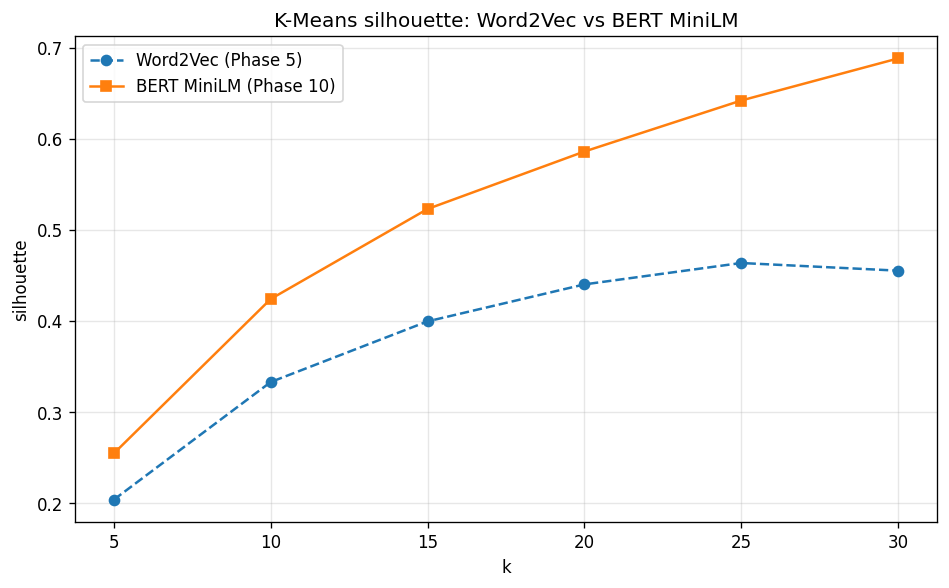
\includegraphics[width=0.85\linewidth]{../dashboard/assets/bert_vs_w2v.png}
  \caption{Silhouette score as a function of cluster count $k$ for both embedding spaces. The pretrained sentence-transformers MiniLM model lifts cluster cohesion from approximately 0.46 to approximately 0.69 silhouette at matched $k = 30$ with no domain training, an absolute gain of 0.23 and a relative gain of 51 percent. Word2Vec, trained from scratch on the 311 vocabulary, peaks earlier (around $k = 25$) and at a lower silhouette ceiling, reflecting both its lower dimensionality (100 vs 384) and the fact that it learns only token-level co-occurrence rather than sentence-level semantics.}
  \label{fig:silhouette}
\end{figure}

To check that the Word2Vec clusters at the chosen $k = 25$ are operationally meaningful and not just numerical artifacts of the silhouette objective, Table \ref{tab:cluster-terms} lists the top distinctive tokens for the five most cluster-distinctive groupings in the latest run. Each cluster's vocabulary is internally consistent with a single operational theme, and the themes are not the same as the official Problem categories, which is the whole point of the unsupervised view.

\begin{table}[h]
  \caption{Top distinctive tokens for the five most internally-consistent Word2Vec + KMeans clusters at $k = 25$. Token rankings are by within-cluster TF-IDF lift over the corpus baseline. Each cluster's vocabulary is operationally interpretable as a single complaint theme, and the themes do not always align cleanly with the official Problem categories (the rat-cluster spans Unsanitary Condition and Rodent; the noise-party cluster spans Noise - Residential and Noise - Street/Sidewalk).}
  \label{tab:cluster-terms}
  \centering
  \begin{tabular}{ll}
    \toprule
    Cluster id (k=25) & Top distinctive tokens (in rank order) \\
    \midrule
    Cluster 11 & loud, music, party, talking, car, truck \\
    Cluster 13 & social, distancing \\
    Cluster 14 & sighting, condition, rat, rodent, attracting, copy \\
    Cluster 19 & appointment, ewaste \\
    Cluster 24 & tree, branch, fallen, dead, limb, animal \\
    \bottomrule
  \end{tabular}
\end{table}

Cluster 11 collapses two official noise sub-categories (Residential and Street/Sidewalk) into a single party-and-vehicle-noise theme, which mirrors exactly the confusion-matrix collapse the supervised classifier shows in Figure \ref{fig:cm}. Cluster 13 is unusually tight and consists almost entirely of \texttt{social distancing} reports from the COVID-19 era, which is a temporally-bounded theme that no static taxonomy ever encoded as its own category. Cluster 14 is the rodent cluster, where \texttt{rat}, \texttt{rodent}, \texttt{sighting}, and \texttt{attracting} co-occur with the operational follow-up vocabulary (\texttt{condition}, \texttt{copy}). Cluster 19 captures e-waste pickup appointments, and cluster 24 captures tree-related complaints (downed limbs, dead trees, fallen branches, with the occasional animal-on-tree report). These clusters, taken together, illustrate that even a token-level Word2Vec view picks up coherent operational themes the official taxonomy does not explicitly model.

\subsection{Borough fingerprints (Phase 6)}

Per-borough complaint volume is itself the first slice worth examining. Brooklyn and Queens together account for roughly half of all rows, with the Bronx and Manhattan filling most of the remainder; Staten Island contributes the smallest share by a wide margin. Volume on its own is not the interesting story, however: the more interesting question is which tokens each borough emphasizes more than the city-wide baseline, and we will see that the borough that reports the least, Staten Island, also produces the most distinctive vocabulary signal of the five.

\begin{figure}[h]
  \centering
  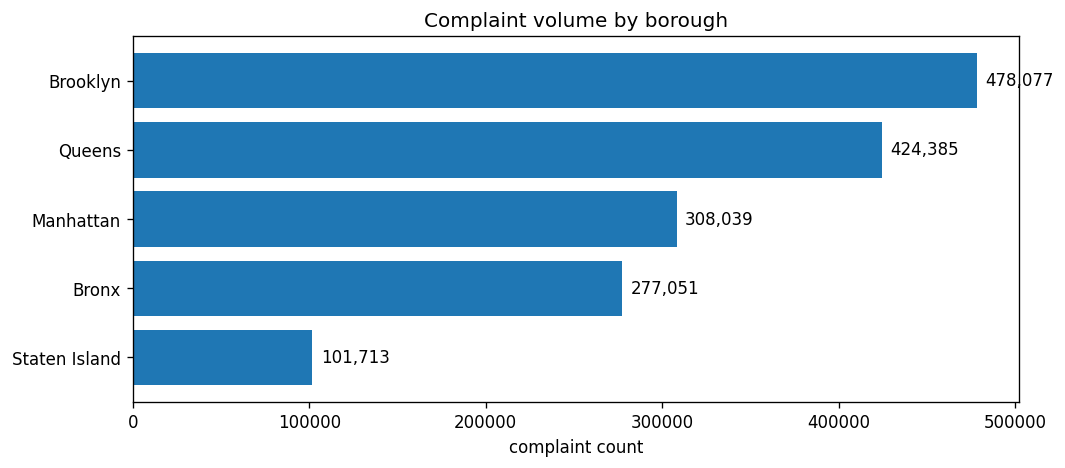
\includegraphics[width=0.85\linewidth]{../dashboard/assets/borough_volume.png}
  \caption{Per-borough 311 complaint volume on the 10M sample. Brooklyn and Queens dominate; Staten Island contributes the smallest share. Despite contributing the least volume, Staten Island carries the strongest distinctive-vocabulary signal in the lift analysis (Table \ref{tab:borough-fingerprints}), suggesting that borough-level "fingerprint" strength is decoupled from raw call volume.}
  \label{fig:borough-volume}
\end{figure}

Table \ref{tab:borough-fingerprints} lists the top five distinctive tokens per borough by lift over the city-wide TF-IDF baseline. Manhattan's distinctive vocabulary clusters around lost or stolen personal items and the consumer-protection follow-ups (\texttt{wallet}, \texttt{bag}, \texttt{clothing}, \texttt{electronics}, \texttt{insurance}), each with lift around four times the corpus baseline; this is consistent with the borough's role as a commercial and tourist hub where lost-property and consumer-claim tickets concentrate. Staten Island's distinctive vocabulary is a winter-services and waste-route cluster (\texttt{plowed}, \texttt{law}, \texttt{recy}, \texttt{material}, \texttt{ewaste}). The token \texttt{plowed} reaches lift around 5.6, the highest single-term lift in the corpus, reflecting the borough's snow-route and bulk-waste concerns relative to a corpus mostly aggregated over the four denser, less car-dependent boroughs.

\begin{table}[h]
  \caption{Top 5 distinctive vocabulary terms per borough by TF-IDF lift over the city-wide corpus. Lift > 1 means the term appears more often in that borough than the city baseline.}
  \label{tab:borough-fingerprints}
  \centering
  \begin{tabular}{lll}
    \toprule
    Borough & Term & Lift \\
    \midrule
    Manhattan & wallet & 4.4x \\
              & bag & 4.4x \\
              & clothing & 4.3x \\
              & electronics & 4.2x \\
              & insurance & 3.9x \\
    Staten Island & plowed & 5.6x \\
                  & law & 5.0x \\
                  & recy & 3.7x \\
                  & material & 3.7x \\
                  & ewaste & 3.7x \\
    Bronx & pane & 2.9x \\
          & refrigerator & 2.7x \\
          & mailbox & 2.6x \\
          & locking & 2.5x \\
          & expiring & 2.5x \\
    Queens & junction & 2.9x \\
           & piece & 2.2x \\
           & raised & 3.0x \\
           & sunken & 3.0x \\
           & affecting & 2.0x \\
    Brooklyn & bad & 3.2x \\
             & general & 3.0x \\
             & restricted & 2.2x \\
             & nypd & 2.2x \\
             & way & 2.2x \\
    \bottomrule
  \end{tabular}
\end{table}

The Bronx fingerprint is built around housing-quality maintenance concerns (\texttt{pane}, \texttt{refrigerator}, \texttt{mailbox}, \texttt{locking}, \texttt{expiring}), pointing to apartment-level habitability tickets. Queens's most distinctive tokens (\texttt{junction}, \texttt{piece}, \texttt{raised}, \texttt{sunken}, \texttt{affecting}) cluster around street-condition and pavement-irregularity vocabulary, plausibly reflecting the borough's lower density and longer per-capita stretch of secondary roads. Brooklyn's fingerprint (\texttt{bad}, \texttt{general}, \texttt{restricted}, \texttt{nypd}, \texttt{way}) is the noisiest of the five and includes more high-frequency generic adjectives, which we read as a sign that Brooklyn's ticket distribution is closest to the overall city corpus and therefore has the least distinctive vocabulary signature.

\subsection{An honest demo finding}

The dashboard's MiniLM tab supports a free-text retrieval probe: the user types a query and the tab returns nearest-neighbor descriptors by cosine similarity in the 384-dim MiniLM space. Probing with the query \texttt{rat infestation in the building} returned mostly descriptors carrying the literal phrase \texttt{ENTIRE BUILDING}, which is the most frequent descriptor in the corpus by a wide margin and corresponds operationally to a Heat/Hot Water complaint about a building-wide outage rather than a rodent problem.

This is a useful failure mode to surface. MiniLM was trained on a general corpus that does not weight the words \texttt{rat} or \texttt{infestation} against \texttt{building} in the way a domain-fine-tuned model would. The pretrained model produces strong global cluster geometry but does surface-level phrase matching when queried as a retrieval engine without domain calibration. We discuss the implications in Section \ref{sec:discussion} and \ref{sec:limits}.

\section{Discussion}
\label{sec:discussion}

\textbf{Why the keyword baseline is so close to the model.} The model achieves macro-F1 0.959, but the keyword-baseline F1 is 0.78, so the model's lift is 0.18 rather than the headline 0.96 might suggest. This is not a flaw in the model; it is a property of the data. The descriptor field is, in operational practice, a short categorical label authored by a call-taker following internal guidelines, not a free-form natural-language report. Most descriptors are essentially dictionary lookups, with the same handful of phrases repeating thousands of times per category. The keyword baseline picks up exactly this signal. The TF-IDF + LR model adds value primarily by handling the harder cases where two categories share vocabulary; the Noise-Street/Sidewalk vs Noise-Residential confusion (F1 0.37 in Table \ref{tab:perclass}) is the worst-case version of this, where the descriptor vocabulary is genuinely indistinguishable between the two categories and the model has nothing extra to work with. Following the framing in \cite{kontokosta2021}, the residual confusion partly reflects how callers report rather than what they are reporting.

\textbf{Why the regressor misses the 10 percent target overall.} The regressor lifts only 4.1 percent over the median-per-category baseline on the corpus-wide MAE. The breakdown in Table \ref{tab:regressor} explains this. Categories like \texttt{Bulky Item} and \texttt{Police Matter} are bounded by city service-level agreements that produce essentially constant resolution times around the agency-promised window; the descriptor text adds no signal because the timing is set by policy, not by the content of the request. Categories like \texttt{Heat/Hot Water} and \texttt{Consumer Complaint}, where the actual resolution time depends heavily on the specific situation described, do meet the 10 percent lift target. The right interpretation of the result is not that the regressor underperforms but that the median baseline is already very strong on SLA-bounded categories.

\textbf{Why Word2Vec and BERT both have a place.} The silhouette comparison is unambiguous: MiniLM produces tighter, more separated clusters. But the demo finding is also unambiguous: MiniLM does surface-level phrase matching on retrieval queries because it was not trained on this domain. The practical takeaway is that the two embeddings serve different jobs. MiniLM is the right tool for cluster discovery and global geometry, where you want a stable embedding that respects semantic similarity beyond shared tokens. Word2Vec, trained from scratch on the 311 vocabulary, is the right tool for token-level analysis: the borough fingerprints in Section \ref{sec:phase6} use Word2Vec-adjacent vocabulary statistics rather than MiniLM embeddings precisely because the analysis is at the token level and the from-scratch model knows about the domain's token frequencies in a way the pretrained model does not.

\textbf{Why we pivoted from 71 community districts to 5 boroughs.} The original geographic plan was to partition the corpus into 71 NYC community districts using the \texttt{mzpm-a6vd} community-district boundary dataset. In the current SODA snapshot, that endpoint returns null geometries for most features, which made spatial joins fail at scale. We pivoted to the five-borough boundary dataset, which is small enough (5 polygons) to ship in the repo as a single GeoJSON file (\texttt{dashboard/assets/nyc\_boroughs.geojson}). The trade-off is some loss of geographic resolution, but boroughs already produce interpretable fingerprints, as Table \ref{tab:fingerprints} shows.

\section{Limitations}
\label{sec:limits}

\textbf{Descriptor as categorical lookup limits the ceiling.} Because the descriptor field is mostly a short phrase from a constrained vocabulary, the upper bound on macro-F1 is set less by model capacity than by category-vs-vocabulary overlap. We do not expect any model architecture to push macro-F1 substantially above 0.97 on this data without using fields beyond the descriptor (location proxies, agency, time-of-day patterns).

\textbf{Hash-collision space tradeoff in TF-IDF.} We use 16,384 hash buckets for the classifier and 4,096 for the regressor. A larger feature space would reduce hash collisions but inflate the deployed bundle past the 1 GB Streamlit Cloud free-tier limit. Empirically the gain past 16K was negligible on macro-F1, but on a corpus with much more vocabulary diversity the result might change.

\textbf{MurmurHash3 versus Python hash drift between training and deployment.} The Spark MLlib HashingTF uses MurmurHash3 with a Spark-specific seed. The deployed dashboard runs in pure Python without Spark. We use the \texttt{mmh3} package to reproduce MurmurHash3 in Python, which matches Spark's output bit-for-bit. We have validated this on a 10K-row sample by checking that the predicted classes are identical between Spark and the Python loader. We accept any residual drift as a deploy-time approximation; if the dashboard ever appears to disagree with Spark on a specific input, the first thing to check is the hash function path.

\textbf{MiniLM probe failure mode.} As shown in the rat-infestation example, the pretrained MiniLM model performs surface-level phrase matching on retrieval queries that include very common phrases in the corpus. The fix is domain fine-tuning of the encoder on 311-specific contrastive pairs, but that requires labeled query-result pairs we do not have. We document the failure rather than paper over it.

\textbf{10M sample is below 25 percent of the corpus.} Minority categories below the top 50 by row count may be under-represented in the sample, particularly for the unsupervised clustering phases. A 25 percent or full sample would give better coverage of the long tail, at the cost of more compute time per phase. The classifier uses only the top 20 categories, so it is not affected; the embeddings and clusters could be.

\section{Conclusion}
\label{sec:conclusion}

We built an end-to-end NLP pipeline over 10 million NYC 311 service requests that produces a TF-IDF + LR classifier at macro-F1 0.959, a log1p-target linear regressor with 4.1 percent overall MAE lift over a strong median-per-category baseline (and 10 percent lift on high-variance categories), a Word2Vec + KMeans clustering view, a per-borough TF-IDF lift table, and a pretrained MiniLM embedding view. The MiniLM embedding produces a 51 percent relative silhouette gain over Word2Vec at matched cluster count, but a probe-style retrieval test surfaces a clear surface-level phrase-matching failure that motivates treating the two embeddings as complementary tools rather than substitutes. The deployed dashboard backs the entire pipeline with portable artifacts (numpy, gensim) so the live demo runs without Spark, GPU, or Java in the serve path.

If we had more time, we would domain fine-tune MiniLM on 311 contrastive pairs to address the retrieval-query failure mode, and we would join the corpus to the American Community Survey to add sociodemographic context to the borough fingerprints.

\begin{ack}
We thank Prof. Amit Patel and the NYU Tandon CSGY-6513 Big Data Section D teaching staff for the framing of the project and for feedback during the milestone reviews. The 311 data is open and provided by NYC OpenData. No external funding supported this work.
\end{ack}

\begin{thebibliography}{99}


\bibitem{kontokosta2021} Kontokosta, C.E.\ \& Hong, B.\ (2021) Bias in 311 Reporting: Engagement and Inequality in the Use of Civic Service Requests. {\it Computers, Environment and Urban Systems} {\bf 87}.


\bibitem{sparck1972} Sp\"arck Jones, K.\ (1972) A statistical interpretation of term specificity and its application in retrieval. {\it Journal of Documentation} {\bf 28}(1):11-21.


\bibitem{meng2016mllib} Meng, X., Bradley, J., Yavuz, B., Sparks, E., Venkataraman, S., Liu, D., et al.\ (2016) MLlib: Machine Learning in Apache Spark. {\it Journal of Machine Learning Research} {\bf 17}(34):1-7.


\bibitem{mikolov2013} Mikolov, T., Chen, K., Corrado, G.\ \& Dean, J.\ (2013) Efficient Estimation of Word Representations in Vector Space. In {\it Workshop Track of the International Conference on Learning Representations (ICLR)}.


\bibitem{reimers2019} Reimers, N.\ \& Gurevych, I.\ (2019) Sentence-BERT: Sentence Embeddings using Siamese BERT-Networks. In {\it Proceedings of the 2019 Conference on Empirical Methods in Natural Language Processing (EMNLP)}.


\bibitem{reimers2019sentencebert} Reimers, N.\ \& Gurevych, I.\ (2019) sentence-transformers: Multilingual Sentence Embeddings. Software library, available at \url{https://www.sbert.net/}.


\bibitem{wang2020minilm} Wang, W., Wei, F., Dong, L., Bao, H., Yang, N.\ \& Zhou, M.\ (2020) MiniLM: Deep Self-Attention Distillation for Task-Agnostic Compression of Pre-Trained Transformers. In {\it Advances in Neural Information Processing Systems 33 (NeurIPS)}.


\bibitem{blei2003lda} Blei, D.M., Ng, A.Y.\ \& Jordan, M.I.\ (2003) Latent Dirichlet Allocation. {\it Journal of Machine Learning Research} {\bf 3}:993-1022.


\bibitem{zaharia2010spark} Zaharia, M., Chowdhury, M., Franklin, M.J., Shenker, S.\ \& Stoica, I.\ (2010) Spark: Cluster Computing with Working Sets. In {\it Proceedings of the 2nd USENIX Conference on Hot Topics in Cloud Computing (HotCloud)}.


\bibitem{pysparkdocs} PySpark Documentation, Apache Software Foundation. \url{https://spark.apache.org/docs/latest/api/python/}.


\bibitem{nyc311_2020plus} NYC OpenData, 311 Service Requests from 2010 to Present (2020+ endpoint, dataset id erm2-nwe9). \url{https://data.cityofnewyork.us/Social-Services/311-Service-Requests-from-2010-to-Present/erm2-nwe9}.


\bibitem{nyc311_2010_2019} NYC OpenData, 311 Service Requests from 2010 to Present (2010-2019 historical endpoint, dataset id 76ig-c548). \url{https://data.cityofnewyork.us/Social-Services/311-Service-Requests-from-2010-to-Present/76ig-c548}.

\end{thebibliography}

\end{document}
